\documentclass[oneside]{ctexbook}

\usepackage{amsmath, amssymb, pgfplots, float}
\pgfplotsset{compat = newest, width = 6cm}
\tikzset{>=latex}

\newcommand\linex[1]{{\draw[thick] (0, #1 / 2) -- (7, #1 / 2); \node at (7.25, #1 / 2) {#1};}}
\newcommand\liney[1]{{\draw[thick] (#1 / 2, 0) -- (#1 / 2, 7); \node at (#1 / 2, -0.25) {#1};}}

\begin{document}
\begin{figure}[H]
	\centering
	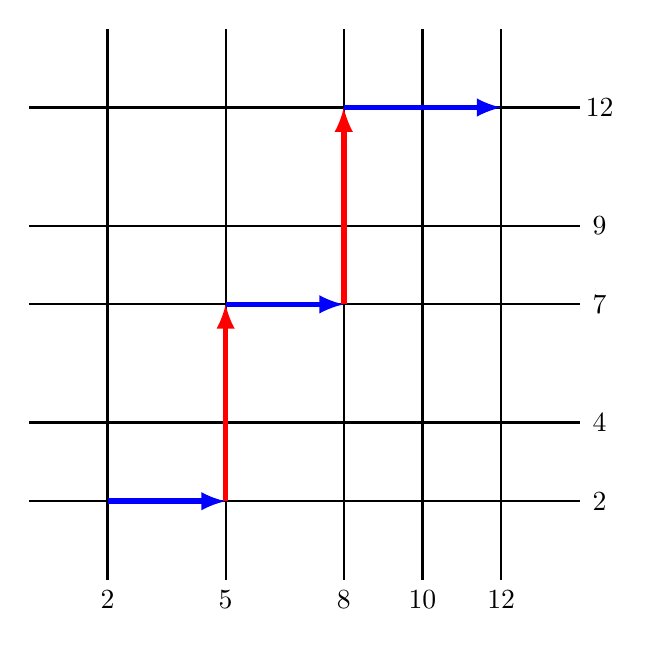
\begin{tikzpicture}
	\linex{2} \linex{4} \linex{7} \linex{9} \linex{12}
	\liney{2} \liney{5} \liney{8} \liney{10} \liney{12}
	\draw[color = blue, ->, line width = 2pt] (2 / 2, 2 / 2) -- (5 / 2, 2 / 2);
	\draw[color = red, ->, line width = 2pt] (5 / 2, 2 / 2) -- (5 / 2, 7 / 2);
	\draw[color = blue, ->, line width = 2pt] (5 / 2, 7 / 2) -- (8 / 2, 7 / 2);
	\draw[color = red, ->, line width = 2pt] (8 / 2, 7 / 2) -- (8 / 2, 12 / 2);
	\draw[color = blue, ->, line width = 2pt] (8 / 2, 12 / 2) -- (12 / 2, 12 / 2);
	\end{tikzpicture}
\end{figure}
\end{document}